\documentclass[a4paper,11pt]{article} % Formato do papel, tipo de documento e tamanho da fonte.
\usepackage[utf8]{inputenc}
\usepackage[brazil]{babel} % Hifenização em português
\usepackage[T1]{fontenc} % Caracteres com acentos são considerados como um bloco
\usepackage{ae} % Arruma a fonte quando usa o pacote acima
\usepackage{amssymb} % Caracteres matemáticos especiais
\usepackage[pdftex]{graphicx} % Para inserir figuras    
\usepackage{indentfirst}
\usepackage{float}

\setlength{\parindent}{1cm}
%\renewcommand{\theenumi}{\Alph{enumi}}

\title{
	\vspace{0 mm}
	\huge{\textbf{MAC0438 - Programação Concorrente}} \\
	\vspace{3 mm}
	\huge{EP2 - Cálculo do número de Euler}
	\vspace{0 mm}
}

\author	{
	\Large{{ Antônio Martins Miranda - Igor Canko Minotto}}	\\
}
\date{\Large{{ 22 de maio de 2014}}}


\usepackage{graphicx}
\begin{document}


\maketitle

\pagebreak 
\tableofcontents

\pagebreak
\setcounter{section}{-1}

\section{Introdução}
  Para calcular o número de Euler, utilizamos a fórmula sugerida: \linebreak 
  \centerline{ $e =\sum\limits_{n=0}^\infty \frac{1}{n!}$ } 
\indent No nosso programa, utilizamos uma thread produtora para calcular os termos da somatória e outras $m-1$ threads consumidoras, sendo $m$ o primeiro argumento da linha de comando. 
  
\section{Ambiente}
  Para rodar os testes que geraram os resultados apresentados neste relatório, usamos o seguinte sistema :
\begin{itemize}
\item SO: Ubuntu Linux 12.04 (32-bit)
\item RAM: 6GB
\item Processador: i5 2.50 GHz x 4 cores
\item Compilador C: gcc 4.6.3
\end{itemize}

\section{Método}
  Demos um valor de entrada 1e-500 ou $10^{-500}$ para o programa, paras as opções f e m. Para medir o tempo de execução,
fizemos a medição dentro do código utilizando a função \textit{clock\_gettime()} da \textit{librt (Realtime Extensions library)}.
Pegamos o valor inicial do relógio no começo da função main, e o valor final logo antes do ponto de retorno da função.
Para cada número de threads, de 1 a 10, foram feitas 1000 repetições. Os resultados se encontram na próxima seção.

\pagebreak
\section{Análise dos Resultados}
  A seguir, vemos os gráficos para as opções m e f, respectivamente:
  \centerline{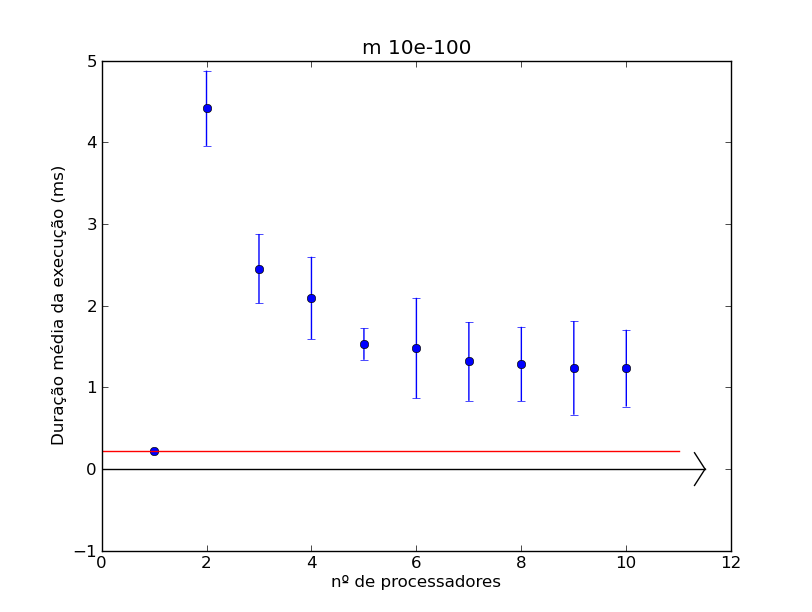
\includegraphics[width=\linewidth]{Dados/m_plot.png}}
  \centerline{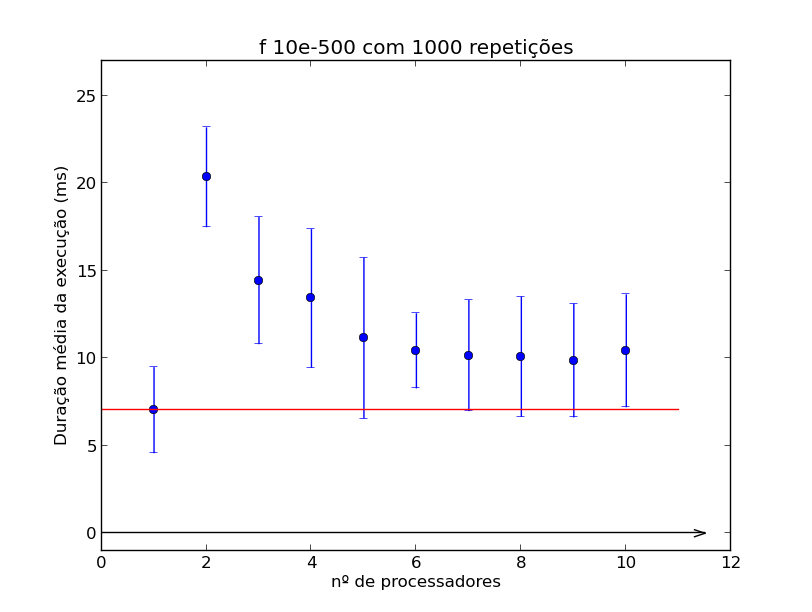
\includegraphics[width=\linewidth]{Dados/f_plot.png}}
  
  \pagebreak 
  \par  Na nossa implementação com threads produtoras e consumidoras, o caso com apenas uma thread deve ser tratado separadamente.
  Assim, a opção s do quarto argumento do programa é equivalente a passar o número 1 como primeiro argumento.
  Isso explica o valor baixo com apenas uma thread, em relação aos outros valores.
  \par
  Ainda assim, criamos uma thread para a execução sequencial. Por que o valor médio do tempo de execução com apenas uma thread
  difere tanto dos outros valores? Isso se deve à nossa implementação, em que utilizamos apenas uma thread produtora, que fica sobrecarregada
  e não consegue produzir tantos termos quanto as threads consumidoras requerem. 
  \par Uma implementação alternativa seria ter um número maior de produtores, para que houvesse um maior equilíbrio
  entre o que é produzido e o que é consumido, reduzindo a espera desnecessária.
  \par Outra opção seria dividirmos o trabalho igualmente entre as threads, mas cada uma calculando os seus próprios termos da somatória, 
  para que não houvesse espera. Mesmo que um mesmo fatorial fosse calculado mais de uma vez, o paralelismo do programa poderia
  compensar em alguma medida esta perda.
  
\end{document}

